

\chapter{Informatie derde vraag}
Deze vraag is een \textbf{oefening}, gequoteerd op 1/2 van de totaalpunten, over één of enkele van volgende onderwerpen:
\begin{itemize}
	\vraag{\accentuate{(1-3)} de Casteljau constructie (van een punt met specifieke parameterwaarde) van een Bézier kromme}{
		\begin{itemize}
			\item Algemeen kan een de Casteljau constructie zoals op figuur \ref{fig:casteljau_construct_1} berekent worden.
			\begin{figure}[ht]
				\centering
				\includegraphics[width=0.6\textwidth]{casteljau_construct_1}
				\caption{Algemene methode de Casteljau constructie.}
				\label{fig:casteljau_construct_1}
			\end{figure}
			Stel nu dat hij de kromme van figuur \ref{fig:casteljau_construct_2} geeft. In dit geval komt $0$ overeen met $a$ en $1$ overeen met $b$. Hij zal enkel nog een willekeurige $t$ waarde geven. Vul het piramidaal schema in met deze $t$, en dan bekom je een gelijkaardige constructie zoals figuur \ref{fig:casteljau_construct_3}.
			\begin{figure}[ht]
				\begin{minipage}{0.5\textwidth}
					\centering
					\includegraphics[width=\textwidth]{casteljau_construct_2}
					\caption{Een Bézier kromme.}
					\label{fig:casteljau_construct_2}
				\end{minipage}
				\begin{minipage}{0.5\textwidth}
					\centering
					\includegraphics[width=\textwidth]{casteljau_construct_3}
					\caption{de Casteljau constructie voor een willekeurige Bézier kromme.}
					\label{fig:casteljau_construct_3}
				\end{minipage}
			\end{figure}
		\end{itemize}			
	}

	\vraag{\accentuate{(1)} verhoging van de graad van Bézier splines (in één enkele stap); voorafgaand moet het verband tussen de \textit{oude} en de \textit{nieuwe} controlepunten opgesteld worden (vermenigvuldiging met een specifieke matrix, cfr. theorieles)}{
		\begin{itemize} 
			\item Eerst algemene formule \accentuate{(niet te kennen)}:
			$$p[u_1, u_2, ... u_m] = \sum_{i_1 = 1}^{m}
			\sum_{\substack{i_2 = 1 \\ i_2 \neq i_1}}^{m}
			...
			\sum_{\substack{i_n = 1 \\ i_n \not\in \{i_1, ... i_{n}\}}}^{m}
			P[{u_i}_1, {u_i}_2, ..., {u_i}_n] \bigg/ \binom{m}{n}
			$$
			Hierbij is $n$ de oude graad en $m$ de nieuwe graad waarbij geldt dat $m > n$. Een verhoging van de graad kan eenvoudig uitgevoerd worden door een matrix met $n + 1$ kolommen en $m + 1$ rijen op te bouwen. Als voorbeeld nemen we een Bézier kromme waarvan we de graad verhogen van 3 naar 6 (dus zeven punten). De matrix kan opgebouwd worden in drie stappen:
			\begin{enumerate}
				\item Een eerste hulpmatrix bevat de binomiale coëfficiënten waarbij een aantal restricties gelden: elke kolom mag slechts $m - n + 1$ niet-nul elementen bevatten, waarbij elke volgende kolom steeds een rij lager begint. Ook moet rekening gehouden dat voor de laatste $n$ rijen $n_i$, $(m-n+2 \leq i \leq m + 1)$ de eerste $i - n - 1$ kolommen vervangen moeten worden door een $0$. Bij ons voorbeeld mag elke kolom slechts $6 - 3 + 1 = 4$ niet-nul elementen bevatten. Bovendien zal rij 5, 6 en 7 respectievelijk beginnen met 1, 2 en 3 nul-elementen.
				$$
				A = 
				\begin{pmatrix}
					1 & 0 & 0  & 0  \\ 
					1 & 1 & 0  & 0  \\ 
					1 & 2 & 1  & 0  \\ 
					1 & 3 & 3  & 1  \\ 
					0 & 4 & 6  & 4  \\ 
					0 & 0 & 10 & 10 \\ 
					0 & 0 & 0  & 20 
				\end{pmatrix}
				$$

				\item Als tweede hulpmatrix nemen we de rotatie van $180$ graden van de eerste matrix:
				$$
				B = 
				\begin{pmatrix}
					20 & 0  & 0 & 0 \\ 
					10 & 10 & 0 & 0 \\ 
					4  & 6  & 4 & 0 \\ 
					1  & 3  & 3 & 1 \\ 
					0  & 1  & 2 & 1 \\ 
					0  & 0  & 1 & 1 \\ 
					0  & 0  & 0 & 1 
				\end{pmatrix}
				$$
				\item Nu kan de effectieve matrix opgesteld worden, door elk element $A_{ij}$ te vermenigvuldigen met elk element $B_{ij}$ \accentuate{(Geen matrixvermenigvuldiging, gewoon de individuele elementen met elkaar vermenigvuldigen)}:
				$$
				C =
				\begin{pmatrix}
					20 & 0  & 0  & 0  \\ 
					10 & 10 & 0  & 0  \\ 
					4  & 12 & 4  & 0  \\ 
					1  & 9  & 9  & 1  \\ 
					0  & 4  & 12 & 4  \\ 
					0  & 0  & 10 & 10 \\ 
					0  & 0  & 0  & 20 
				\end{pmatrix}
				$$
			\end{enumerate}
		
			Deze matrix kan nu eenvoudig vermenigvuldigt worden met de rijmatrix van de originele punten $P(t)$ om de nieuwe punten $Q(t)$ te bekomen. Elke kolom stelt één van de originele 4 punten voor. Een punt $Q_i$ kan hieruit afgeleidt worden door op de $i$-de rij, de som van 
			de producten van het originele punt met de factor voor die kolom te berekenen, en deze som te delen door $\binom{m}{n}$. In dit geval is $m = 6$ en $n = 3$, zodat $\binom{6}{3} = \frac{6!}{3! 3!} = 20$. De zeven punten worden dus:
			$$
			\begin{pmatrix}
				Q_{000000} (=Q_0) \\
				Q_{000001} (=Q_1)\\
				Q_{000011} (=Q_2)\\
				Q_{000111} (=Q_3)\\
				Q_{001111} (=Q_4)\\
				Q_{011111} (=Q_5)\\
				Q_{111111} (=Q_6)\\
			\end{pmatrix}
			= 
			\frac{1}{20}
			\begin{pmatrix}
				20 & 0  & 0  & 0  \\ 
				10 & 10 & 0  & 0  \\ 
				4  & 12 & 4  & 0  \\ 
				1  & 9  & 9  & 1  \\ 
				0  & 4  & 12 & 4  \\ 
				0  & 0  & 10 & 10 \\ 
				0  & 0  & 0  & 20 
			\end{pmatrix}
			\cdot 
			\begin{pmatrix}
				P_{000} (=P_0)\\
				P_{001} (=P_1)\\
				P_{011} (=P_2)\\
				P_{111} (=P_3)\\
			\end{pmatrix}
			$$
			\begin{itemize}
				\item $Q_0 = \frac{1}{20} (20P_0 + 0P_1  + 0P_2  + 0P_3) = P_0$
				\item $Q_1 = \frac{1}{20}(10P_0 + 10P_1 + 0P_2  + 0P_3) = \frac{1}{2}(P_0 + P_1)$ 
				\item $Q_2 = \frac{1}{20}(4P_0  + 12P_1 + 4P_2  + 0P_3) = \frac{1}{5}(P_0  + 3P_1 + P_2)$
				\item $Q_3 = \frac{1}{20}(1P_0  + 9P_1 + 9P_2  + 1P_3) = \frac{1}{20}(P_0 + 9P_1  + 9P_2 + P_3)$
				\item $Q_4 = \frac{1}{20}(0P_0  + 4P_1 + 12P_2  + 4P_3) = \frac{1}{5}(P_1  + 3P_2 + P_3)$
				\item $Q_5 = \frac{1}{20}(0P_0  + 0P_1 + 10P_2  + 10P_3) = \frac{1}{2}(P_2 + P_3)$
				\item $Q_6 = \frac{1}{20}(0P_0  + 0P_1 + 0P_2  + 20P_3) = P_3$
			\end{itemize}
			
			\begin{itemize}
				\item De punten $Q_0$ en $Q_6$ komen respectievelijk overeen met $P_0$ en $P_3$ en moeten niet gewijzigd worden.
				\item Voor de punten $Q_1$ en $Q_5$ passen we respectievelijk $1/2$ af tussen $P_0$ en $P_1$ en tussen $P_2$ en $P_3$.
				\item Voor het punt $Q_2$ passen we eerst een hulppunt $R$ af op $1/5$ van het punt $P_1$. Van $R$ naar $P_{2}$ zetten we het punt $Q_2$ op $1/5$ van $R$.
			\end{itemize}
		\end{itemize}}
	\vraag{\accentuate{(2)} verhoging van de graad van Bézier splines (\textit{stapsgewijs}: één graad verhogen per stap)}{
		\begin{itemize} 
			\item Slechts één graad verhogen per stap is heel eenvoudig:
			      $$Q_k = \frac{k}{n + 1}P_{k - 1} + \frac{n + 1 - k}{n + 1}P_k$$
			      Stel een bézierkromme van de 3de graad met punten $P_{000}, P_{001}, P_{011}$ en $P_{111}$.
			      			
			      De nieuwe punten van de bézierkromme van de 4de graad worden dan:
			      \begin{itemize}
			      	\item $Q_{0000} =\frac{3 + 1 - 0}{3 + 1}P_{00} = P_{000}$
			      	\item $Q_{0001} = \frac{1}{4}P_{000} + \frac{4 - 1}{4}P_{001} = \frac{1}{4}P_{000} + \frac{3}{4}P_{001}$
			      	\item $Q_{0011} = \frac{1}{2}P_{001} + \frac{1}{2}P_{011}$
			      	\item $Q_{0111} = \frac{3}{4}P_{011} + \frac{1}{4}P_{111}$
			      	\item $Q_{1111} = P_{111}$
			      \end{itemize}
			      Het punt $Q_{0001}$ ligt bijvoorbeeld op het punt waarvoor $t=0.75$ op het lijnstuk $[P_{000}P_{001}]$.
		\end{itemize}}

	\vraag{\accentuate{(3,4)} segmentering (subdivisie) van Bézier krommen (eventueel meerdere segmenten in één enkele stap)}
		{
			\begin{itemize} 
				\item Als je een de Casteljau constructie toepast op een Bézier kromme, introduceer je hulppunten, die perfect kunnen dienen als de nieuwe punten van twee of meerdere bézierkrommen. Bekijk figuur \ref{fig:subdivision_1}, waarbij de Bézierkromme gegeven wordt door de punten $(P_{0000}, P_{0001},$ $P_{0011}, P_{0111}, P_{1111})$. Het kan onmiddelijk gesegmenteerd worded in twee bézier krommen, respectievelijk bepaald door $(P_{0000},P_{000t},P_{00tt},P_{0ttt},P_{tttt})$ en $(P_{tttt},P_{ttt1},P_{tt11},P_{t111},P_{1111})$. Het is ook mogelijk om kubieke Bézierkrommen in meerdere segmenten op te splitsen, zoals te zien op figuur \ref{fig:subdivision_2}, die respectievelijk segmenten bepalen door $(P_{000}, P_{00s}, P_{0ss}, P_{sss})$, $(P_{sss}, P_{sst}, P_{stt}, P_{ttt})$ en $(P_{ttt}, P_{tt1}, P_{t11}, P_{111})$. 
				\begin{figure}[ht]
					\begin{minipage}{0.5\textwidth}
						\centering
						\includegraphics[width=\textwidth]{subdivision_1}
						\caption{Een bézierkromme van graad vier.}
						\label{fig:subdivision_1}
					\end{minipage}
					\begin{minipage}{0.5\textwidth}
						\centering
						\includegraphics[width=\textwidth]{subdivision_2}
						\caption{Een kubieke bézierkromme van graad drie.}
						\label{fig:subdivision_2}
					\end{minipage}

				\end{figure}
			
			\end{itemize}
		}
	\vraag{\accentuate{(9-10,14-16)} constructie van de \textit{kromtecirkel} in een punt van een Bézier kromme}
	{
		\begin{itemize} 
			\item Algemene methode om een kromtecirkel te berekenen in een punt van een Bézier kromme wordt weergegeven op figuur \ref{fig:kromtecirkel}. De kromming van een Bézier kromme wordt bepaald door de hulppunten van de laatste 2 iteraties van het de Casteljau proces. Eerst moet dus een de Casteljau constructie uitgevoerd worden op de Bézier kromme voor het opgegeven punt $t$. De straal $R$ van de kromtecirkel wordt gegeven door $$R = \frac{3\Delta^2}{4\delta}$$
			Het volgende proces kan op twee manieren uitgevoerd worden, hier doe ik het voor de controlepunten $(P_{00t}, P_{0tt})$, maar zou evengoed gelden voor de controlepunten $(P_{tt1}, P_{t11})$. De afstand van $P_{ttt}$ tot $P_{0tt}$ noemen we $\Delta_0$ \accentuate{(is vrij onbelangrijk, maar toch vermeld ik het omdat het op de figuur staat)}. Het lijnstuk dat samenvallend is met $|P_{ttt}P_{0tt}|$ moet doorgetrokken worden, zodanig dat er een rechte hoek gemaakt kan worden tussen het eindpunt van dit lijnstuk en het punt $P_{00t}$. De afstand van $P_{00t}$ en dit eindpunt noemen we $\delta_0$. Nu kunnen we een lijnstuk, loodrecht op het lijnstuk $|P_{0tt}P_{tt1}|$ en door het punt $P_{ttt}$ met lengte $\frac{4}{3} \delta_0$ tekenen. Op dit moment kan er vanuit $P_{0tt}$ een lijnstuk getrokken worden tot aan het einde van het vorige lijnstuk, gevolgd door een ander lijnstuk, loodrecht met het vorige lijnstuk, zodanig dat het kruist met het verlengde van het lijnstuk door $P_{ttt}$. Deze kruising is het middelpunt van de cirkel. De afstand van dit middelpunt tot $P_{ttt}$ is de straal $R$ van de cirkel.
			
			\begin{figure}[ht]
				\centering
				\includegraphics[width=\textwidth]{kromtecirkel}
				\caption{De kromtecirkel door het punt $P_{ttt}$.}
				\label{fig:kromtecirkel}
			\end{figure}
		\end{itemize}
			
		}
	\vraag{\accentuate{(5-7,9-11)} constructie van de \textit{Bézier representatie} van een (polynomiale) NURBS}{
		\begin{itemize}
			\item De knooppunten van de B-spline worden datapunten van de Bézier-representatie. Deze vraag wordt opgelost met het voorbeeld op figuur \ref{fig:bezier_repr_polynomiale_nurbs_1}.
			\begin{figure}[ht]
				\centering
				\includegraphics[width=0.5\textwidth]{bezier_repr_polynomiale_nurbs_1}	
				\caption{Fase 1 bézier representatie van een polynomiale NURBS.}
				\label{fig:bezier_repr_polynomiale_nurbs_1}
			\end{figure}

			De knopenvector wordt gegeven: $(-1, 0, 1 ; 2, 3, 3, 4, 5, 6, 7, 7, 7, 8, 9 ; 9, 9, 9)$. Wat meteen opvalt is dat er 7 (waarvan sommige hogere multipliciteit) reële knooppunten zijn, wat betekent dat de resulterende bézier spline 6 segmenten zal bevatten. Schrijf eerst de blossomnotatie van elk knooppunt, zoals weergegeven op figuur \ref {fig:bezier_repr_polynomiale_nurbs_2}.
			\begin{figure}[ht]
				\centering
				\includegraphics[width=0.5\textwidth]{bezier_repr_polynomiale_nurbs_2}	
				\caption{Fase 2 bézier representatie van een polynomiale NURBS.}
				\label{fig:bezier_repr_polynomiale_nurbs_2}
			\end{figure}

			Via de multilineariteit eigenschap kan men nieuwe punten introduceren. (\accentuate{herhaling op figuur \ref{fig:multilineariteit}})
			\begin{figure}[ht]
				\centering
				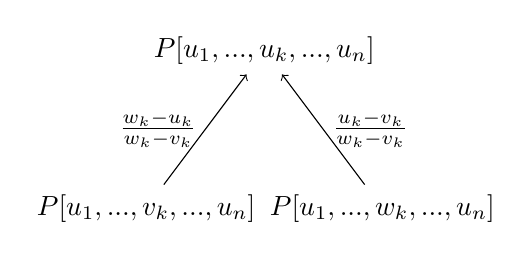
\begin{tikzpicture}
					\node (x) at (0, 0) {$P[u_1,...,v_k,...,u_n]$};
					\node (z) at (1.5, 2) {$P[u_1,...,u_k,...,u_n]$};
					\node (y)at (3, 0) {$P[u_1,...,w_k,...,u_n]$};

					\draw[->] (x) -- node[xshift=-0.6cm]{$\frac{w_k - u_k}{w_k - v_k}$} (z);
					\draw[->] (y) -- node[xshift=0.6cm]{$\frac{u_k - v_k}{w_k - v_k}$} (z);
				\end{tikzpicture}
				\caption{Multilineariteit eigenschap.}
				\label{fig:multilineariteit}
			\end{figure}	

			Bijvoorbeeld: tussen punt 012 en 123 moeten nog twee hulppunten komen: 112 en 122. Stel in het diagram $u_k = 1, v_k = 0$ en $w_k = 2$. dan krijgen we
			$$P[1,1,2] = \frac{2}{3}P[0,1,2] + \frac{1}{3}P[1,2,3]$$
			of anders gezegd: het punt 112 ligt op $t = 1/3$ voor het lijnstuk $[P[0,1,2]P[1,2,3]]$.
			Analoog voor $u_k = 2, v_k = 0$ en $w_k = 2$, dan krijgen we
			$$P[1,2,2] = \frac{1}{3}P[0,1,2] + \frac{2}{3}P[1,2,3]$$
			of anders gezegd: het punt 122 ligt op $t = 2/3$ voor het lijnstuk  $[P[0,1,2]P[1,2,3]]$.
			Als je dit zou doen voor punten 123 en 233, dan zou je 
			$$P[2, 2, 3] = \frac{1}{2}P[1,2,3] + \frac{1}{2}P[2,3,3]$$
			krijgen, zodat het punt 223 mooi in het midden van het lijnstuk $[P[1,2,3]P[2,3,3]]$ ligt. Een leuke eigenschap is, dat als de knopenvector geen gaten vertoond, dat het lijnstuk altijd mooi opgesplitst wordt. Als je op een lijnstuk dan 2 hulppunten moet introduceren, zal het eerste punt op $1/3$ van het lijnstuk liggen, en het tweede punt op $2/3$. Als je 3 hulppunten moet introduceren, zal het eerste punt op $1/4$ van het lijnstuk liggen, enz... Een voorbeeld van een knopenvector met gaten, waardoor je dus best manueel uitrekend, is $(0, 1, 3 ; 4, 6 ; 7, 9, 10)$. Alle nieuwe hulppunten kunnen zo berekend worden, en is te zien op figuur \ref{fig:bezier_repr_polynomiale_nurbs_3}.
			\begin{figure}[ht]
				\centering
				\includegraphics[width=0.5\textwidth]{bezier_repr_polynomiale_nurbs_3}	
				\caption{Fase 3 bézier representatie van een polynomiale NURBS.}
				\label{fig:bezier_repr_polynomiale_nurbs_3}
			\end{figure}

			Punten waarvan slechts 1 argument van de blossomnotatie verschillen, en die op een ander lijnstuk liggen, kunnen geïnterpoleerd worden. Teken een lijnstuk door elk paar punten waarvoor dit van toepassing is. Op figuur \ref{fig:bezier_repr_polynomiale_nurbs_4} wordt dit uitgewerkt, samen met het introduceren van de nieuwe hulppunten.
			\begin{figure}[ht]
				\centering
				\includegraphics[width=0.5\textwidth]{bezier_repr_polynomiale_nurbs_4}	
				\caption{Fase 4 bézier representatie van een polynomiale NURBS.}
				\label{fig:bezier_repr_polynomiale_nurbs_4}
			\end{figure}

			Tot slot moeten nog enkel de punten verbonden worden waarvan de blossomnotatie bestaat uit een herhaling van slechts één argument. In dit voorbeeld zijn dat de punten 222, 333, 444, 555, 666, 777, 888 en 999. Zoek eerst in de knopenvector op of er knooppunten zijn met een hogere multipliciteit. \accentuate{De continuïteit in een knooppunt horend bij een knoop met multipliciteit $\mu$ wordt gegeven door $C^{k - 1 - \mu}$}.
			
			Het knooppunt 3 heeft een multipliciteit van 2, zodat slechts $C^{4 - 1 - 2} = C^1$ continuïteit voldaan is. Het knooppunt 7 heeft een multipliciteit van 3, zodat daar slechts $C^0$ voldaan is. Dit is belangrijk bij het tekenen van de kromme, zoals te zien op figuur \ref{fig:bezier_repr_polynomiale_nurbs_5}.
			\begin{figure}[ht]
				\centering
				\includegraphics[width=0.5\textwidth]{bezier_repr_polynomiale_nurbs_5}	
				\caption{Fase 5 bézier representatie van een polynomiale NURBS.}
				\label{fig:bezier_repr_polynomiale_nurbs_5}
			\end{figure}
		\end{itemize}}
	\vraag{\accentuate{(6-10)} constructie van controlepunten na toevoeging van één of meerdere \textit{reële} knopen in de knopenvector van een (polynomiale) NURBS (zonder over te gaan op de Bézier representatie)}
	{
		\begin{itemize} 
			\item Voeg het nieuwe punt zoveel keer toe als de multipliciteit van de knoop aangeeft in de knopenvector. Daarna moeten er zoveel iterataties van het algoritme van de Boor uitgevoerd worden als de multipliciteit van de nieuwe knoop. Figuur \ref{fig:bspline_toevoeging_rk_m1}, \ref{fig:bspline_toevoeging_rk_m2} en \ref{fig:bspline_toevoeging_rk_m3} geven respectievelijk het toevoegen van een knoop met multipliciteit 1, 2 of 3 weer.
			\begin{figure}[ht]
				\begin{minipage}{0.5\textwidth}
					\centering
					\includegraphics[width=\textwidth]{bspline_toevoeging_rk_m1}	
					\caption{Knoop toevoegen met multiplicteit 1 bij een NURBS van graad 3.}
					\label{fig:bspline_toevoeging_rk_m1}
				\end{minipage}
				\begin{minipage}{0.5\textwidth}
					\centering
					\includegraphics[width=\textwidth]{bspline_toevoeging_rk_m2}	
					\caption{Knoop toevoegen met multiplicteit 2 NURBS van graad 3.}
					\label{fig:bspline_toevoeging_rk_m2}
				\end{minipage}
			\end{figure}
			\begin{figure}[ht]
				\centering
				\includegraphics[width=0.7\textwidth]{bspline_toevoeging_rk_m3}	
				\caption{Knoop toevoegen met multiplicteit 3 NURBS van graad 3.}
				\label{fig:bspline_toevoeging_rk_m3}
			\end{figure}
		\end{itemize}
	}
	\vraag{\accentuate{(10)} constructie van controlepunten na toevoeging van één of meerdere \textit{virtuele} knopen in de knopenvector van een (polynomiale) NURBS (zonder over te gaan op de Bézier representatie)}{
		\begin{itemize} 
			\item Als de toe te voegen virtuele knoop de meest extreme virtuele knoop wordt, dan vervangen we de meest extreme virtuele knoop met deze nieuwe knoop en blijven alle andere controlepunten ongewijzigd aangezien geen enkel van de controlepunten afhankelijk is van de meest extreme virtuele knoop. 
			$$(t_0, t_1, t_2, ..., t_{k - 2} ; t_{k - 1}, t_k, t_{k + 1}, ...) \rightarrow (t_x, t_1, t_2, ..., t_{k - 2} ; t_{k - 1}, t_k, t_{k + 1}, ...)$$

			\item In het andere geval moeten de virtuele knopen opgeschoven worden tot dat de virtuele knoop op zijn plaats zit:
			$$(t_0, t_1, t_2, ..., t_j, t_{j + 1}, ..., t_{k - 2} ; t_{k - 1}, t_k, t_{k + 1}, ...) \rightarrow (t_1, t_2, ..., t_j, t_x, t_{j + 1}, ..., t_{k - 2} ; t_{k - 1}, t_k, t_{k + 1}, ...)$$
			Hierbij worden er $j$ virtuele knopen opgeschoven, en moeten ook $j$ controlepunten vervangen worden. Voer hiervoor het algoritme van de Boor op, met als basis van het schema de  ??? \todo{niet gevonden}
		\end{itemize}
	}
	\vraag{\accentuate{(11)} berekening en constructie van de controlepunten van de \textit{open-uniforme} representatie van een (polynomiale) NURBS met een \textit{uniforme} knopenvector}
	{
		\begin{itemize} 
			\item Bij een uniforme knopenvector vormen alle knopen een rekenkundige rij. Bij een open-uniforme knopenvector vormen enkel de reële knopen een rekenkundige rij. De meest extreme reële knopen worden $k$ maal herhaald. 

			Zo wordt de uniforme knopenvector $\{-1, 0, 1; 2, 3, 4, 5 ; 6, 7, 8 \}$ in open-uniforme vorm: $\{2, 2, 2; 2, 3, 4, 5; 5, 5, 5\}$. 

			Een open-uniforme NURBS begint en eindigt op respectievelijk het eerste en laatste datapunt.
		\end{itemize}
	}
	\vraag{\accentuate{(12,19)} berekening en constructie van de controlepunten van de \textit{uniforme} representatie van een polynomiale of rationale NURBS met een \textit{open-uniforme} knopenvector}{\begin{itemize} \item \todo{oplossen} \end{itemize}}
	\vraag{\accentuate{(12)} de Boor constructie (van een punt met specifieke parameterwaarde) van een (polynomiale) NURBS}
	{
		\begin{itemize} 
			\item Hierbij wordt een piramidaal schema gebruikt dat bijna identiek is aan het schema dat gebruikt wordt voor het algoritme van de Casteljau. Het verschil is hier echter dat bij elke iteratie hetzelfde vervangend argument, $t$, wordt geïntroduceerd, zoals te zien op figuur \ref{fig:deboor_constructie}.

			\begin{figure}[ht]
				\centering
				\includegraphics[width=0.7\textwidth]{deboor_constructie}
				\caption{de Boor constructie.}
				\label{fig:deboor_constructie}
			\end{figure}
		\end{itemize}
		}
	\vraag{\accentuate{(13)} constructie van de \textit{hodograaf} van een Bézier kromme of spline}
	{
		\begin{itemize}
			\item Stel het schema van de Casteljau op voor de gegeven Bézierkromme, maar voer in de eerste stap de blokken van het afgeleide type in, zoals weergegeven op figuur \ref{fig:constructie_hodograaf}. De resulterende hodograaf is zelf een Bézierkrommme van een graad minder en wordt gegeven door de resterende blokken van het interpolerende type.
			\begin{figure}[ht]
				\centering
				\includegraphics[width=0.6\textwidth]{constructie_hodograaf}	
				\caption{Constructie van het de Casteljau schema voor een hodograaf.}
				\label{fig:constructie_hodograaf}
			\end{figure}
		\end{itemize}
		
	}
	\vraag{\accentuate{(13-16)} vaststellen van de continuïteit in de knooppunten van Bézier splines (\textit{stelling van Stärk})}
	{
		\begin{itemize} 
		\item \textbf{Stelling van Stärk:} Men bereikt $C^k$ continuïteit indien de blossomargumenten voor elk van de $2k$ naburige controlepunten hetzelfde punt in de ruimte oplevert, of men nu de argumenten evalueert in de blossompolynoom van het ene segment, of in de blossompolynoom van het andere segment. 
		\item Veronderstel een linkersegment met data- en controlepunten $P[a, a, a], P[a, a, b], P[a, b, b]$ en $P[b, b, b]$, en een rechtersegment, bepaald door $Q[b, b, b], Q[b, b, c], Q[b, c, c]$ en $Q[c, c, c]$ met gemeenschappelijk punt $P[b, b, b] \equiv Q[b, b, b]$. Dit is ook te zien op figuur \ref{fig:stark_1}.
		\begin{figure}[ht]
			\centering
			\includegraphics[width=\textwidth]{stark_1}
			\caption{Een Bézier spline.}
			\label{fig:stark_1}
		\end{figure}
		
		Aangezien we dit gemeenschappelijk punt hebben is $C^0$ continuïteit voldaan. Om $C^1$ continuïteit te bereiken moet, indien men de argumenten van controlepunt $P[a, b, b]$ van het linkersegment evalueert in de blossom van het rechtersegment, dit een punt $Q[a, b, b]$ opleveren dat samenvalt met $P[a, b, b]$. Hetzelfde moet gelden tussen controlepunt $Q[b,b,c]$ van het rechtersegment, en het punt $P[b,b,c]$ van het linkersegment, bekomen door de argumenten te evalueren in de blossom van het linkersegment. Om $C^2$ continuïteit te hebben doet men hetzelfde voor punten $P[a,a,b]$ en $Q[b,c,c]$. Om $C^3$ continuïteit te hebben doet men hetzelfde voor punten $P[a,a,a]$ en $Q[c,c,c]$. Dit is te zien op figuur \ref{fig:stark_2}.

		\begin{figure}[ht]
			\centering
			\includegraphics[width=\textwidth]{stark_2}
			\caption{De stelling van Stärk.}
			\label{fig:stark_2}
		\end{figure}
			
		\end{itemize}
	}
	\vraag{\accentuate{(17)} constructie van de controlepunten van de \textit{uniforme} Lagrange representatie van een Lagrange geïnterpoleerde kromme met \textit{niet-uniforme} knopenvector; schematisch aantonen hoe de berekening van de Bézier representatie van deze kromme zou kunnen uitgevoerd worden (ondermeer opstellen van de \textit{inverse} van de Bézier basismatrix).}{
		\begin{itemize} 
			\item x
			\item De matrix voor een Bézierkromme van willekeurige graad $n$ kan als volgt opgesteld worden:
				\begin{enumerate}
					\item Construeer de driehoek van Pascal, in de linkerbovenhoek van een $(n + 1) \cdot (n + 1)$ matrix, vertrekkend van de rechterbovenhoek. De overige coëfficiënten blijven nul.
					\item Vermenigvuldig alle coëfficiënten van kolom $j$, met de coëfficiënt in rij $j$ van de eerste kolom.
					\item Keer het teken om van alle coëfficiënten op de even nevendiagonalen. 
				\end{enumerate}
				Toegepast op de figuur \accentuate{($n = 3$ aangezien 4 datapunten)}:
				$$
				\begin{pmatrix}
					-1 & 3 & -3 & 1 \\
					3 & -6 & 3 & 0 \\
					-3 & 3 & 0 & 0 \\
					1& 0 & 0 & 0
				\end{pmatrix}
				$$
			\newpage
		\end{itemize}}
		
	\vraag{\accentuate{(18,19)} constructie van een  \textit{benadering door lijnstukken} van een uniforme NURBS door toepassing van het algoritme van Lane \& Riesenfeld}{
		\begin{itemize} 
			\item Dit is een eenvoudig iteratief proces: pas altijd de helft af tussen twee punten, zoals te zien op figuur \ref{fig:lane_and_riesenfeld}.
			\begin{figure}[ht]
				\centering
				\includegraphics[width=0.6\textwidth]{lane_and_riesenfeld}	
				\caption{Het algoritme van Lane en Riesenfeld.}
				\label{fig:lane_and_riesenfeld}
			\end{figure}
			

		\end{itemize}}
	\vraag{\accentuate{(20)} constructie van een \textit{triangulair schema} met behulp van het veralgemeend algoritme van Neville (voor een specifieke configuratie van inputgegevens), en berekening hieruit van de \textit{gewichtsfuncties} en de \textit{matrixrepresentatie}}{
		\begin{itemize} 
			\item \accentuate{Het veralgmeend algoritme van Neville laat toe om de rekenregels van Hermite interpolatie op te stellen, aangezien Hermite interpolatie ook nog gebruik maakt van richtingsvectoren en eventueel krommingen, die gedefinieerd worden op hetzelfde punt, zodat het punt een hogere multipliciteit krijgt. Hermite interpolatie gebruikt slechts twee datapunten $P_0$ en $P_1$, waarvoor men meestal respectievelijk $t=0$ en $t=1$ neemt}. Bij het veralgemeend algoritme van Neville zijn er twee mogelijkheden:
				\begin{enumerate}
					\item Indien er minstens twee verschillende indices in $P_{pqr...wxy}(t)$ optreden, dan blijft de traditionele versie van het algoritme onveranderd geldig, zoals te zien op figuur \ref{fig:hermite_interpolation_1}.
					\begin{figure}[ht]
						\centering
						\includegraphics[width=0.5\textwidth]{hermite_interpolation_1}
						\caption{Lineaire interpolatie met het algoritme van Neville.}
						\label{fig:hermite_interpolation_1}
					\end{figure}	
					\item Indien echter in de labeling van een hulppunt, of van het eindresultaat, slechts één enkele index $i$ optreedt, met multipliciteit $\mu_i = m + 1$, dan moet op het lager niveau slechts één enkel hulppunt geïntroduceerd worden: het hulppunt waarin de index $i$ optreedt met multipliciteit $\mu_i = m$. Ter  vervanging van lineaire interpolatie moet nu gebruik gemaakt worden van Taylor reeksontwikkelingen, zoals te zien op figuur \ref{fig:hermite_interpolation_2}.
					\begin{figure}[ht]
						\centering
						\includegraphics[width=0.5\textwidth]{hermite_interpolation_2}
						\caption{Taylor reeksontwikkeling met het algoritme van Neville.}
						\label{fig:hermite_interpolation_2}
					\end{figure}	
						
				\end{enumerate}
				Veronderstel nu een Hermite interpolatie van graad drie. Dit heeft twee datapunten $P_0$ en $P_1$ en de richtingsvectoren in deze punten $P_0^{'}$ en $P_1^{'}$. Punt $P_{0011}(t)$ is de top van het piramidaal schema. Op figuur \ref{fig:20triangular} wordt dit schema voorgesteld.

				\begin{figure}[ht]
					\centering
					\includegraphics[width=\textwidth]{hermite_interpolation_3}
					\caption{Constructie van het triangulair schema.}
					\label{fig:20triangular}
				\end{figure}
				De gewichtsfuncties kunnen berekent worden via de volgende stappen:
				\begin{enumerate}
					\item Keer elke pijl van het schema om.
					\item Plaats de constante 1 op de top van de piramide.
					\item De mengfunctie horend bij een specifiek basisdatapunt $P_i$, kan bekomen worden door in het aangepaste diagram achtereenvolgens:
						\begin{enumerate}
							\item het aantal alternatieve paden te zoeken die tot dit punt leiden (eenvoudig via de driehoek van Pascal),
							\item de gewichtsfactoren langs een specifiek pad te vermenigvuldigen,
							\item de bijdrage van elk individueel pad te sommeren.
						\end{enumerate}
				\end{enumerate}
		
				Op figuur \ref{fig:20invtriangular} wordt het omgekeerde schema getoond.
		
				\begin{figure}[ht]
					\centering
					\includegraphics[width=\textwidth]{hermite_interpolation_4}
					\caption{Het inverse triangulair schema dat op figuur \ref{fig:20triangular} geconstrueerd werd.}
					\label{fig:20invtriangular}
				\end{figure}
				
				De mengfuncties worden dan:
				\begin{equation*}
					\begin{split}
						H_{1, 3}(t)  & = \bigg[{\color{red}t}(1-t)^2\bigg] = t^3 -2t^2 + t \\
						H_{0, 3}(t)  & = \bigg[{\color{red}1}(1-t)^2 + 2(1-t)^2{\color{blue}t}\bigg]= 2t^3 - 3t^2 + 1\\
						H_{3, 3}(t)  & = \bigg[{\color{blue}t^2} + 2{\color{blue}t^2}(1-t)\bigg] = -2t^3 + 3t^2\\
						H_{2, 3}(t)  & = \bigg[{\color{blue}t^2}{\color{red}(t-1)}\bigg] = t^3 - t^2
					\end{split}
				\end{equation*}
				Omgevormd tot de matrixrepresentatie:
				$$
				P(t) = (t^3, t^2, t, 1) 
				\cdot
				\begin{pmatrix}
					2 & -2 & 1 & 1 \\
					-3 & 3 & -2 & -1 \\
					0 & 0 & 1 & 0 \\
					1 & 0 & 0 & 0
				\end{pmatrix}
				\cdot 
				\begin{pmatrix}
					P_0 \\
					P_1 \\
					P_0^{'} \\
					P_1^{'} \\
				\end{pmatrix}
				$$
				\accentuate{CONTROLE: Som van de waarden van de rijen voor elk datapunt moet 0 zijn: $-24 -12 - \frac{1}{2} + \frac{1}{2} + a_4 + a_5 = 0 $}.
		
		\end{itemize}}



			
\end{itemize}